\section{Equilibration}
It is important that we allow the system to equilibrate before we can trust our data. We can tell that our simulation has equilibrated when there is no longer a time drift in any of our observables. In figs. \ref{fig:pres}, \ref{fig:temp}, and \ref{fig:energy} we plot our observables over 1000 timesteps in order to see the cessation in drift in our observables.
\begin{figure}[h]
\minipage{0.5\textwidth}
  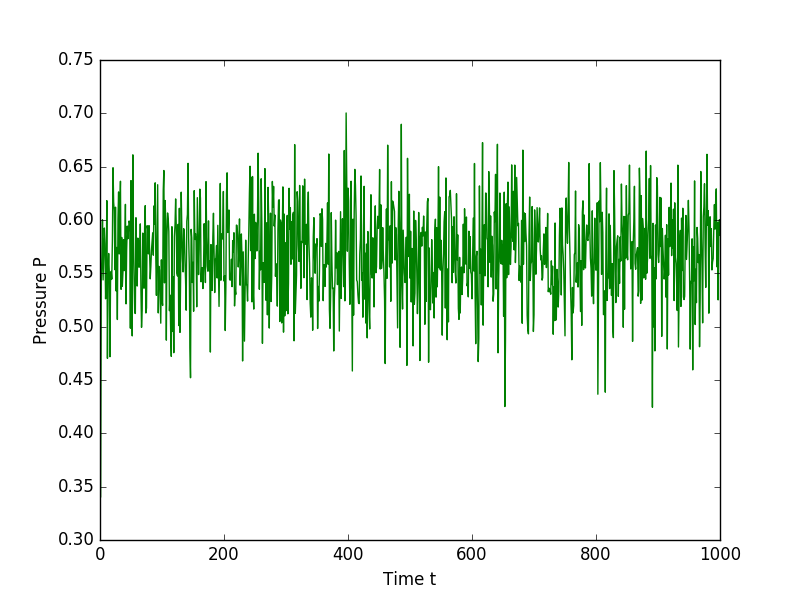
\includegraphics[width=\linewidth]{fig/Pressure.png}
  \caption{Pressure plotted over 1000 timesteps}\label{fig:pres}
\endminipage\hfill
\minipage{0.5\textwidth}
  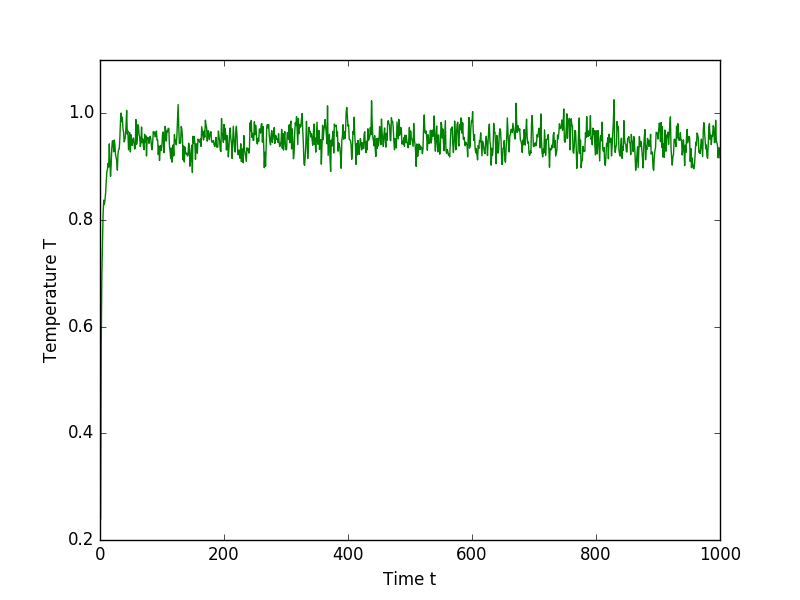
\includegraphics[width=\linewidth]{fig/Temperature.png}
  \caption{Temperature plotted over 1000 timesteps}\label{fig:temp}
\endminipage
\end{figure}
\begin{figure}[h]
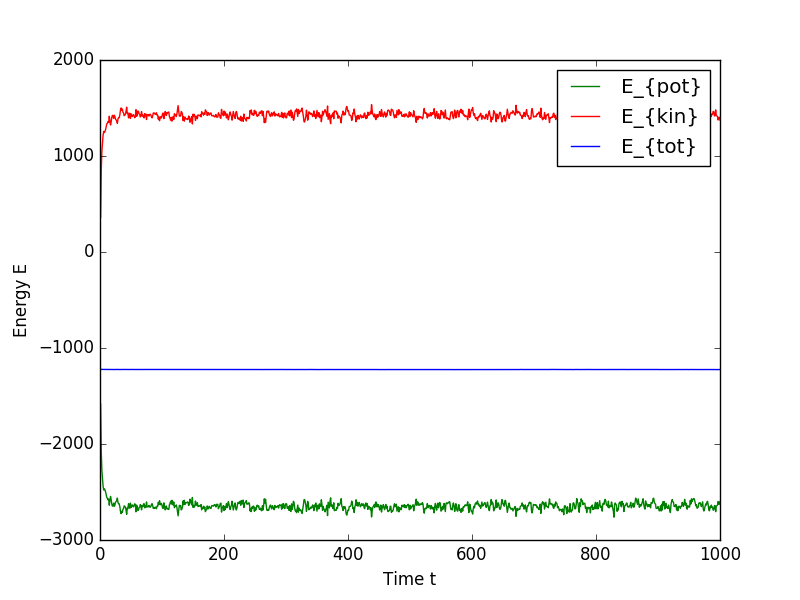
\includegraphics[width=0.7\linewidth]{fig/Energies.png}
  \centering
  \caption{Energy plotted over 1000 timesteps.}
\label{fig:energy}
\end{figure}

In order to smooth out these plots we would like to compute the running average of the observables. This is given by
\begin{equation}
\hat{O}_i = \frac{1}{M+1} \sum_{i - M/2}^{i+M/2} O_i
\end{equation}
where $M$ is the window size of the average. We implemented the running average in python in the file ljanalyze.py.
\listfile{../src/ljanalyze.py}{src/ljanalyze.py}{33}{42}{Running Average}{5ave}
Figures \ref{fig:pres1}, \ref{fig:temp1}, and \ref{fig:energy1} show the running averages with $M$ = 10 and figures \ref{fig:pres2}, \ref{fig:temp2}, and \ref{fig:energy2} show the running averages with $M$ = 100. All three observables seem to equilibrate within 100 timesteps. The pressure starts close to equilibrium so that its fluctuations are larger than the initial equilibration. The temperature also quickly equilibrates but changes from a much different nonequilibrium state. The energies quickly exchange between kinetic and potential before coming to equilibrium. Our plots make it clear that 200 timesteps is plenty of time to allow the system to eq	uilibrate.
\begin{figure}[h]
\minipage{0.32\textwidth}
  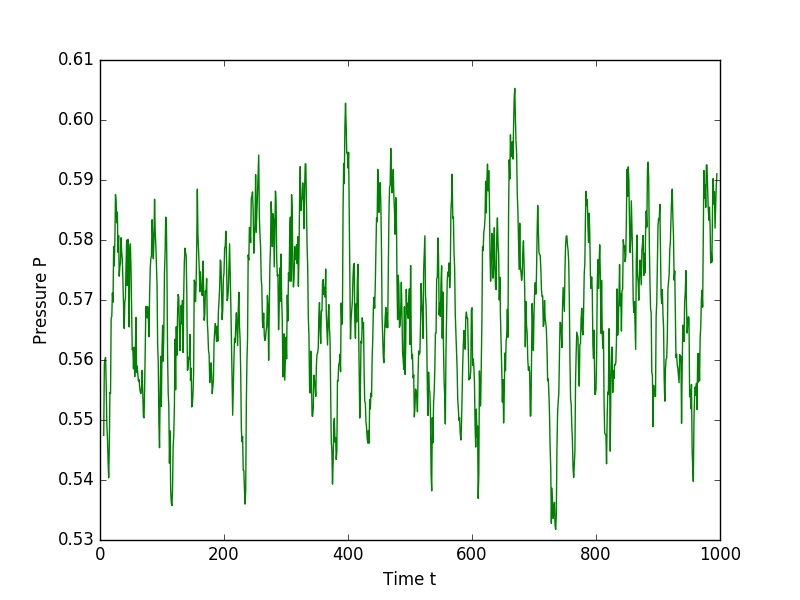
\includegraphics[width=\linewidth]{fig/avPressure_M10.png}
  \caption{Running average of pressure with M = 10}\label{fig:pres1}
\endminipage\hfill
\minipage{0.32\textwidth}
  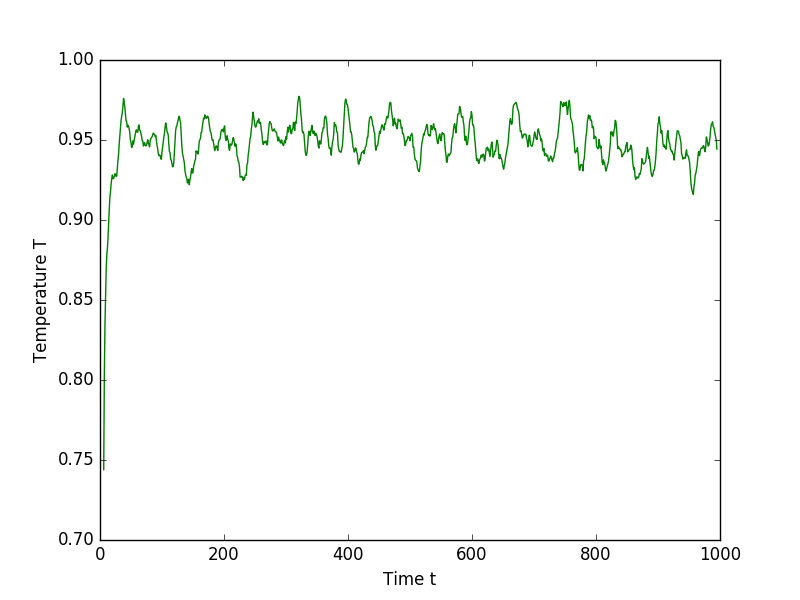
\includegraphics[width=\linewidth]{fig/avTemperature_M10.png}
  \caption{Running average of temperature with M = 10}\label{fig:temp1}
\endminipage\hfill
\minipage{0.32\textwidth}
  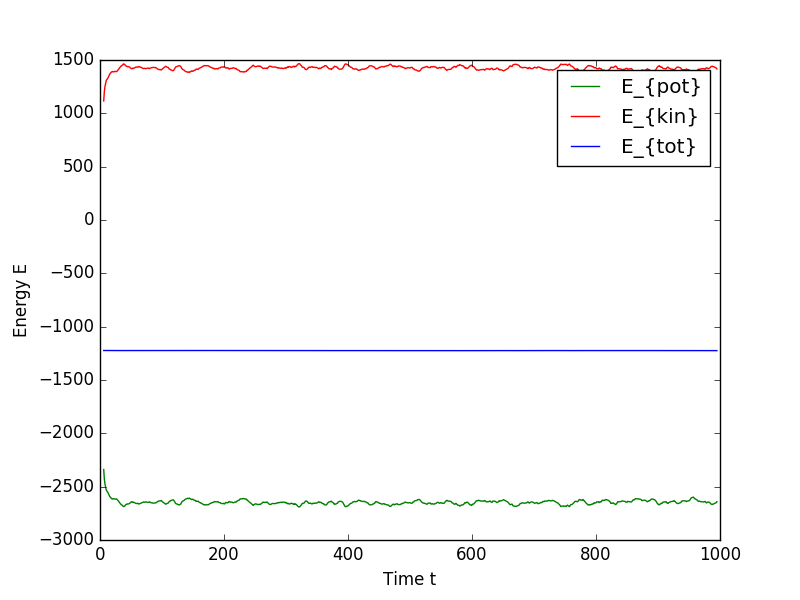
\includegraphics[width=\linewidth]{fig/avEnergies_M10.png}
  \caption{Running average of energy with M = 10}\label{fig:energy1}
\endminipage
\end{figure}

Finally, we extend ljanalyze.py to compute the average value of the observables after equilibration. This is done with the following function.
\listfile{../src/ljanalyze.py}{src/ljanalyze.py}{44}{49}{Compute Mean}{5mean}
We pass the number of timesteps needed for equilibration in with a command line argument and our code returns the mean values.
In our case we measured $E_\mathrm{pot} = -2652.8$, $E_\mathrm{kin} = 1427.8$, $E_\mathrm{tot} = -1225.0$, $T = 0.952$, and $P = 0.568$.

\begin{figure}[h]
\minipage{0.32\textwidth}
  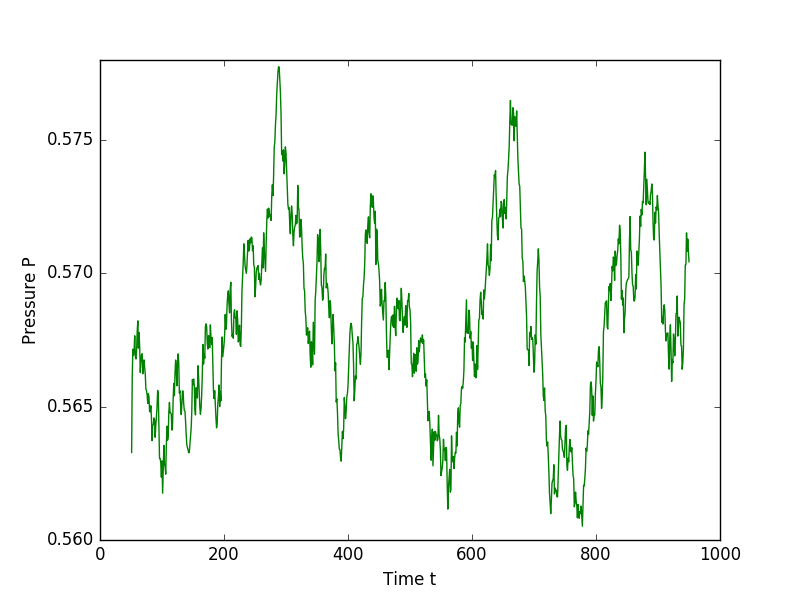
\includegraphics[width=\linewidth]{fig/avPressure_M100.png}
  \caption{Running average of pressure with M = 100}\label{fig:pres2}
\endminipage\hfill
\minipage{0.32\textwidth}
  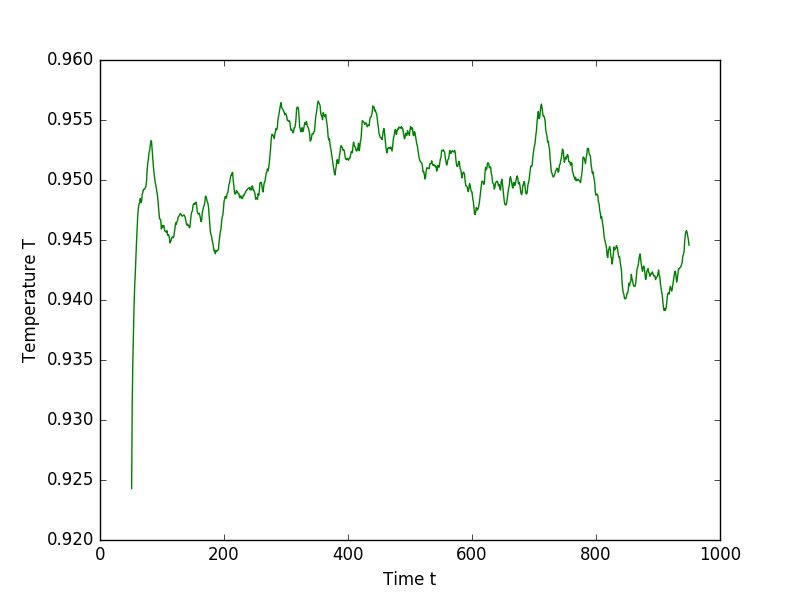
\includegraphics[width=\linewidth]{fig/avTemperature_M100.png}
  \caption{Running average of temperature with M = 100}\label{fig:temp2}
\endminipage\hfill
\minipage{0.32\textwidth}
  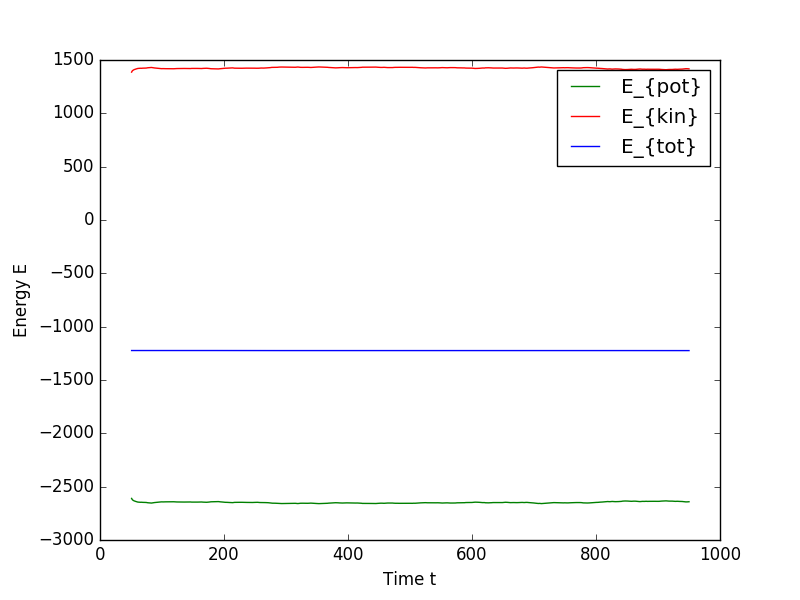
\includegraphics[width=\linewidth]{fig/avEnergies_M100.png}
  \caption{Running average of energy with M = 100}\label{fig:energy2}
\endminipage
\end{figure}
